\begin{figure*}
\centering
\hfill
\begin{subfigure}{0.15\linewidth}
\fbox{\includegraphics[width=0.8\linewidth]{../data/patchinput}}
\caption{}
\label{fig:apples-a}
\end{subfigure}
\hfill
\begin{subfigure}{0.15\linewidth}
\fbox{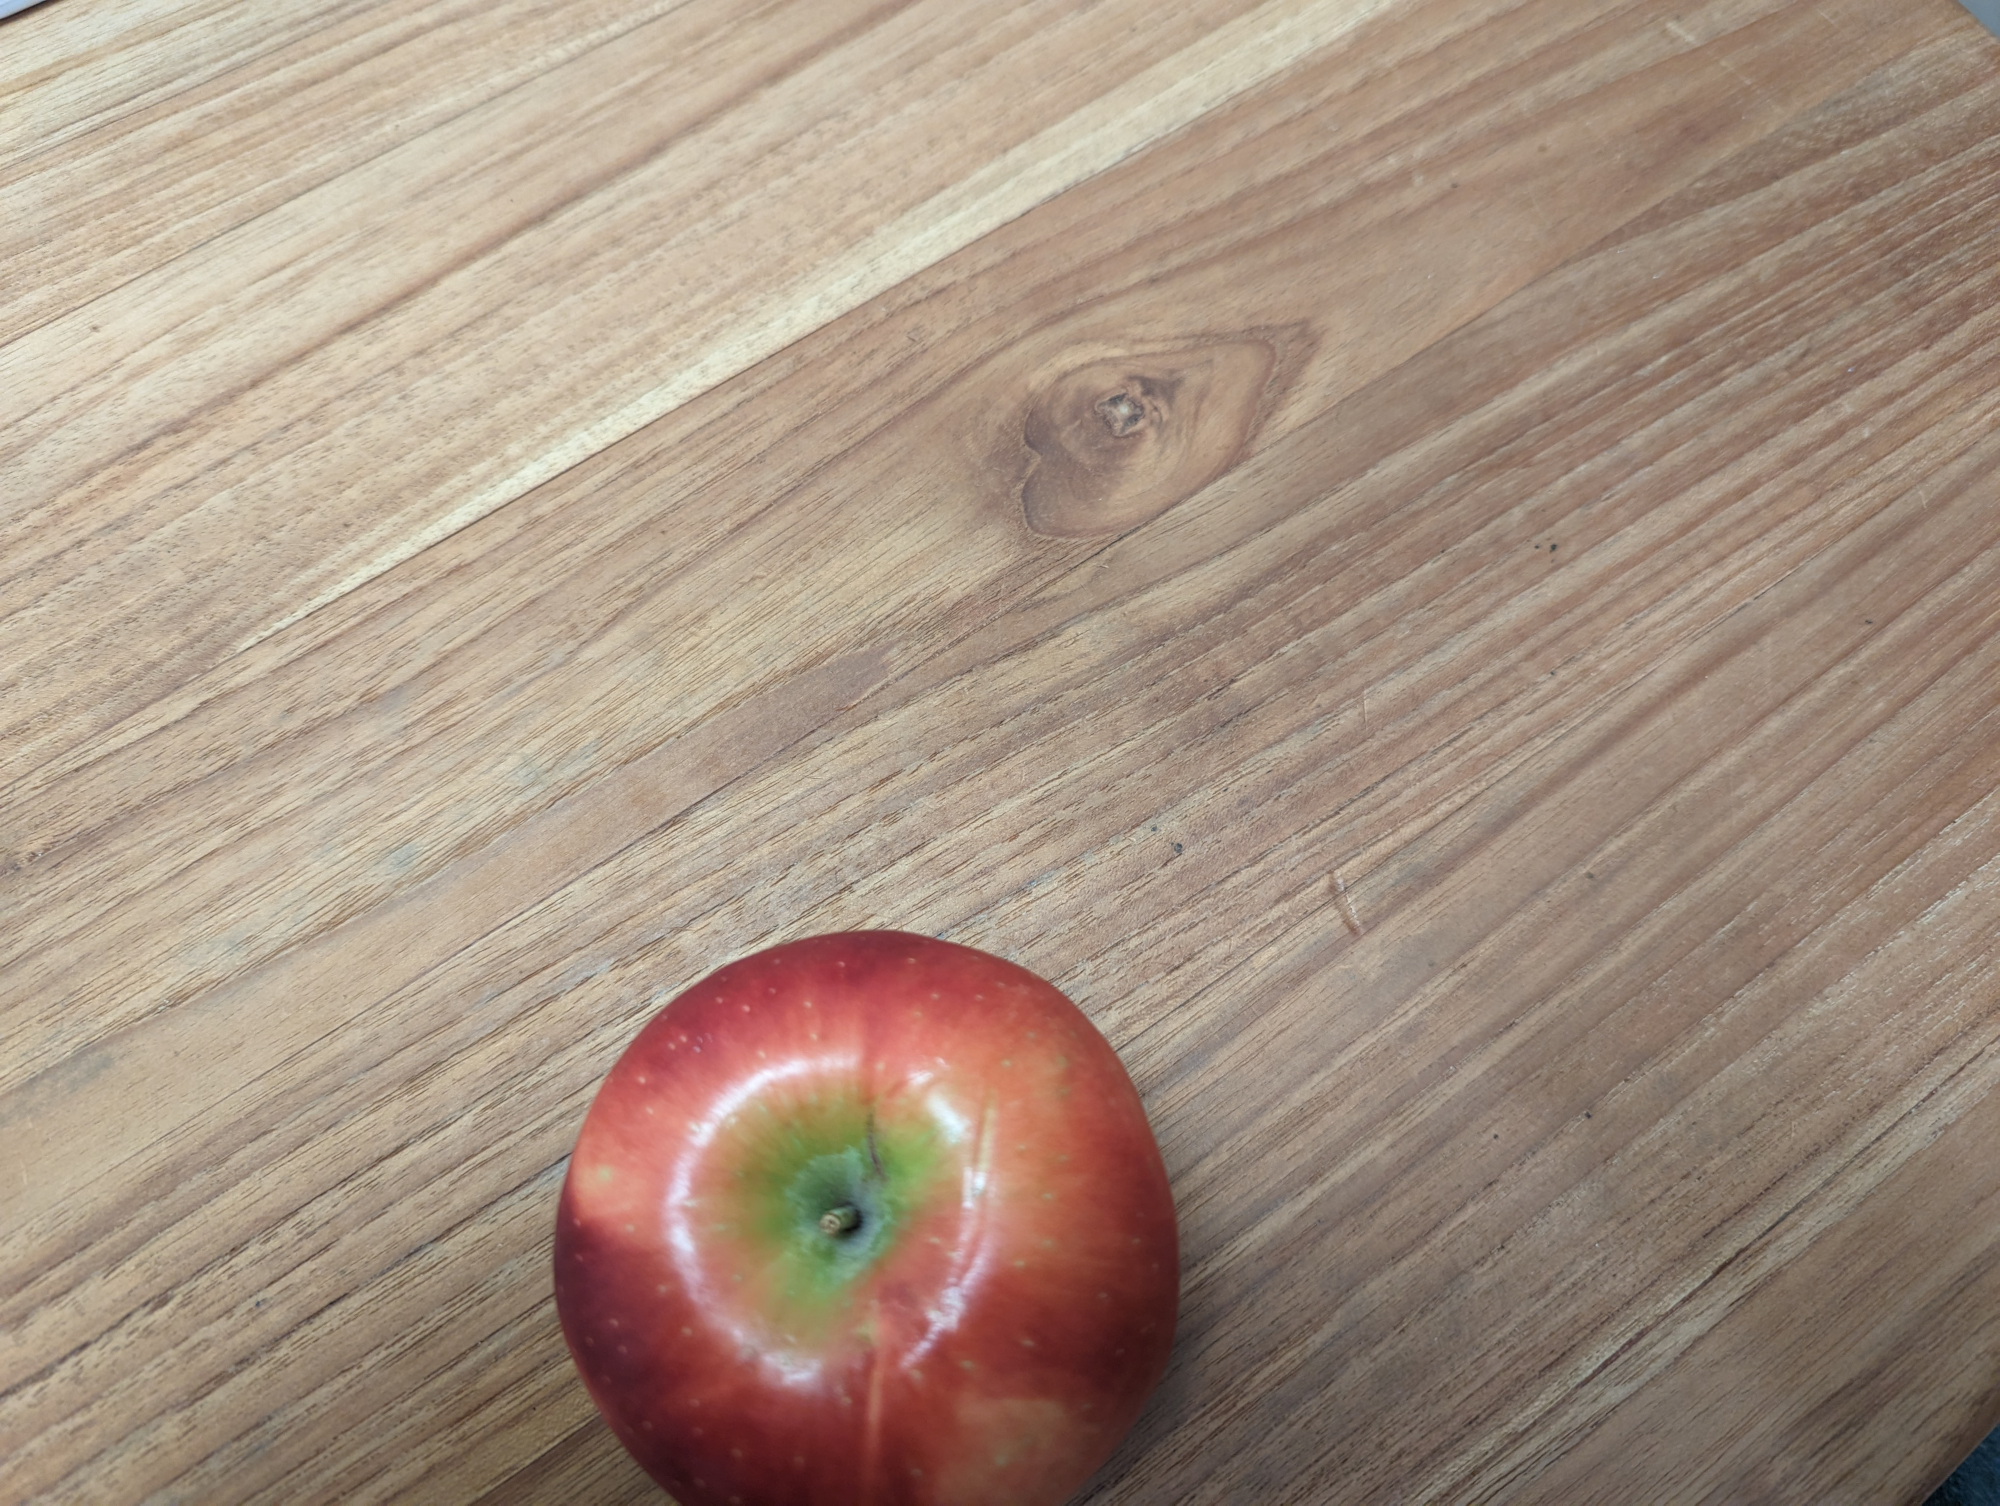
\includegraphics[width=0.8\linewidth]{../data/patchrefs/ref2}}
\caption{}
\label{fig:apples-b}
\end{subfigure}
\hfill
\begin{subfigure}{0.15\linewidth}
\fbox{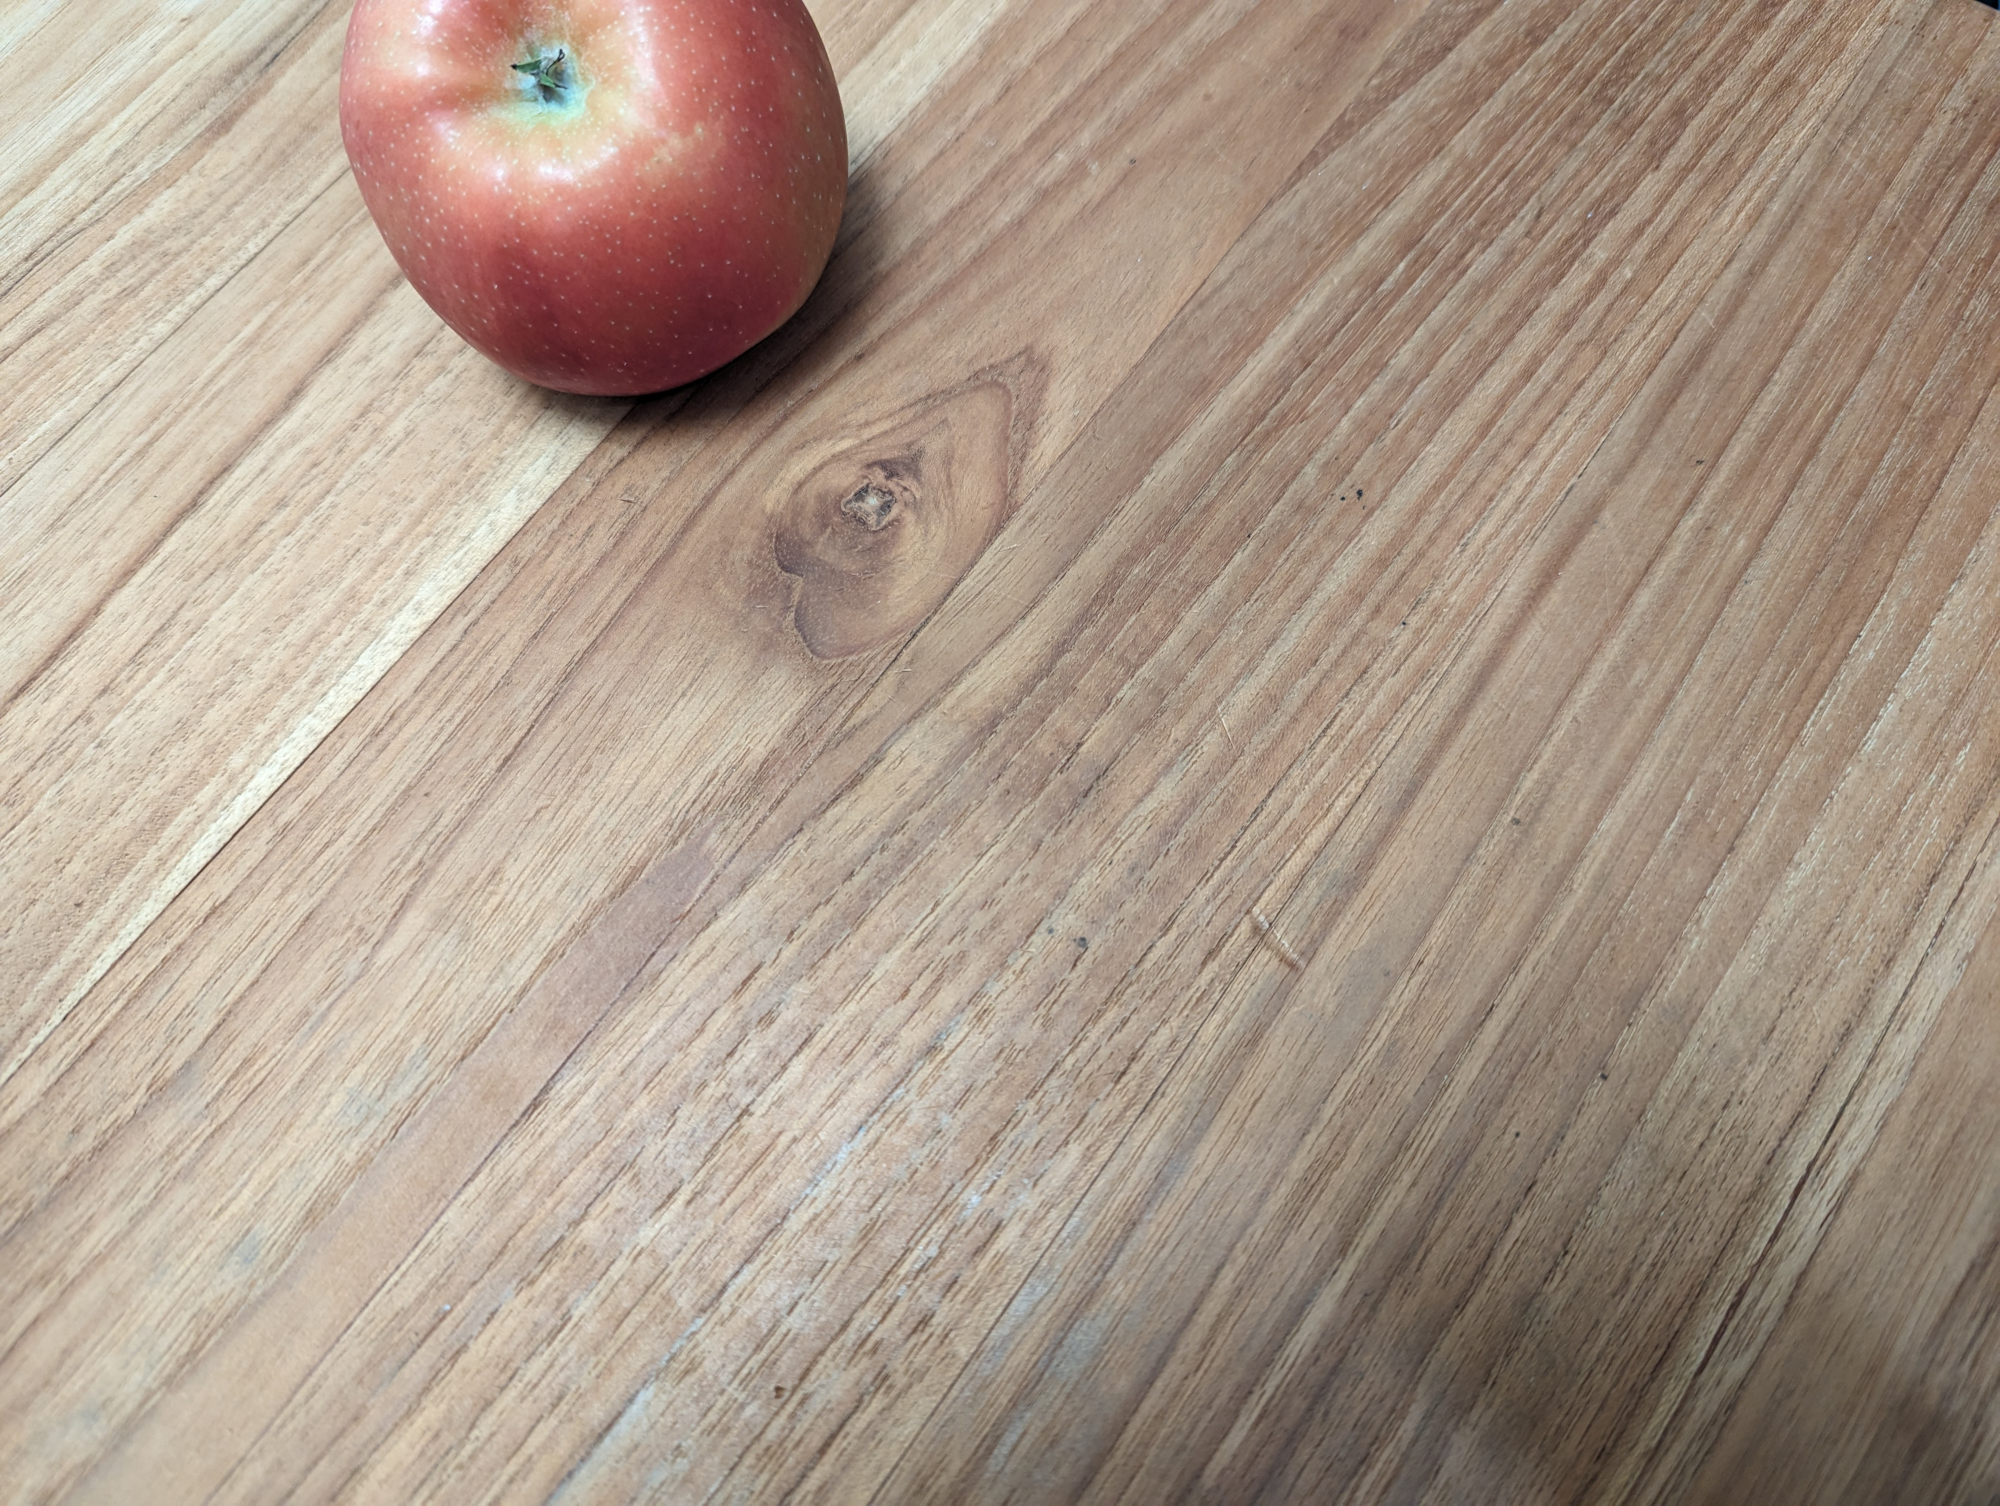
\includegraphics[width=0.8\linewidth]{../data/patchrefs/ref3}}
\caption{}
\label{fig:apples-c}
\end{subfigure}
\hfill
\begin{subfigure}{0.15\linewidth}
\fbox{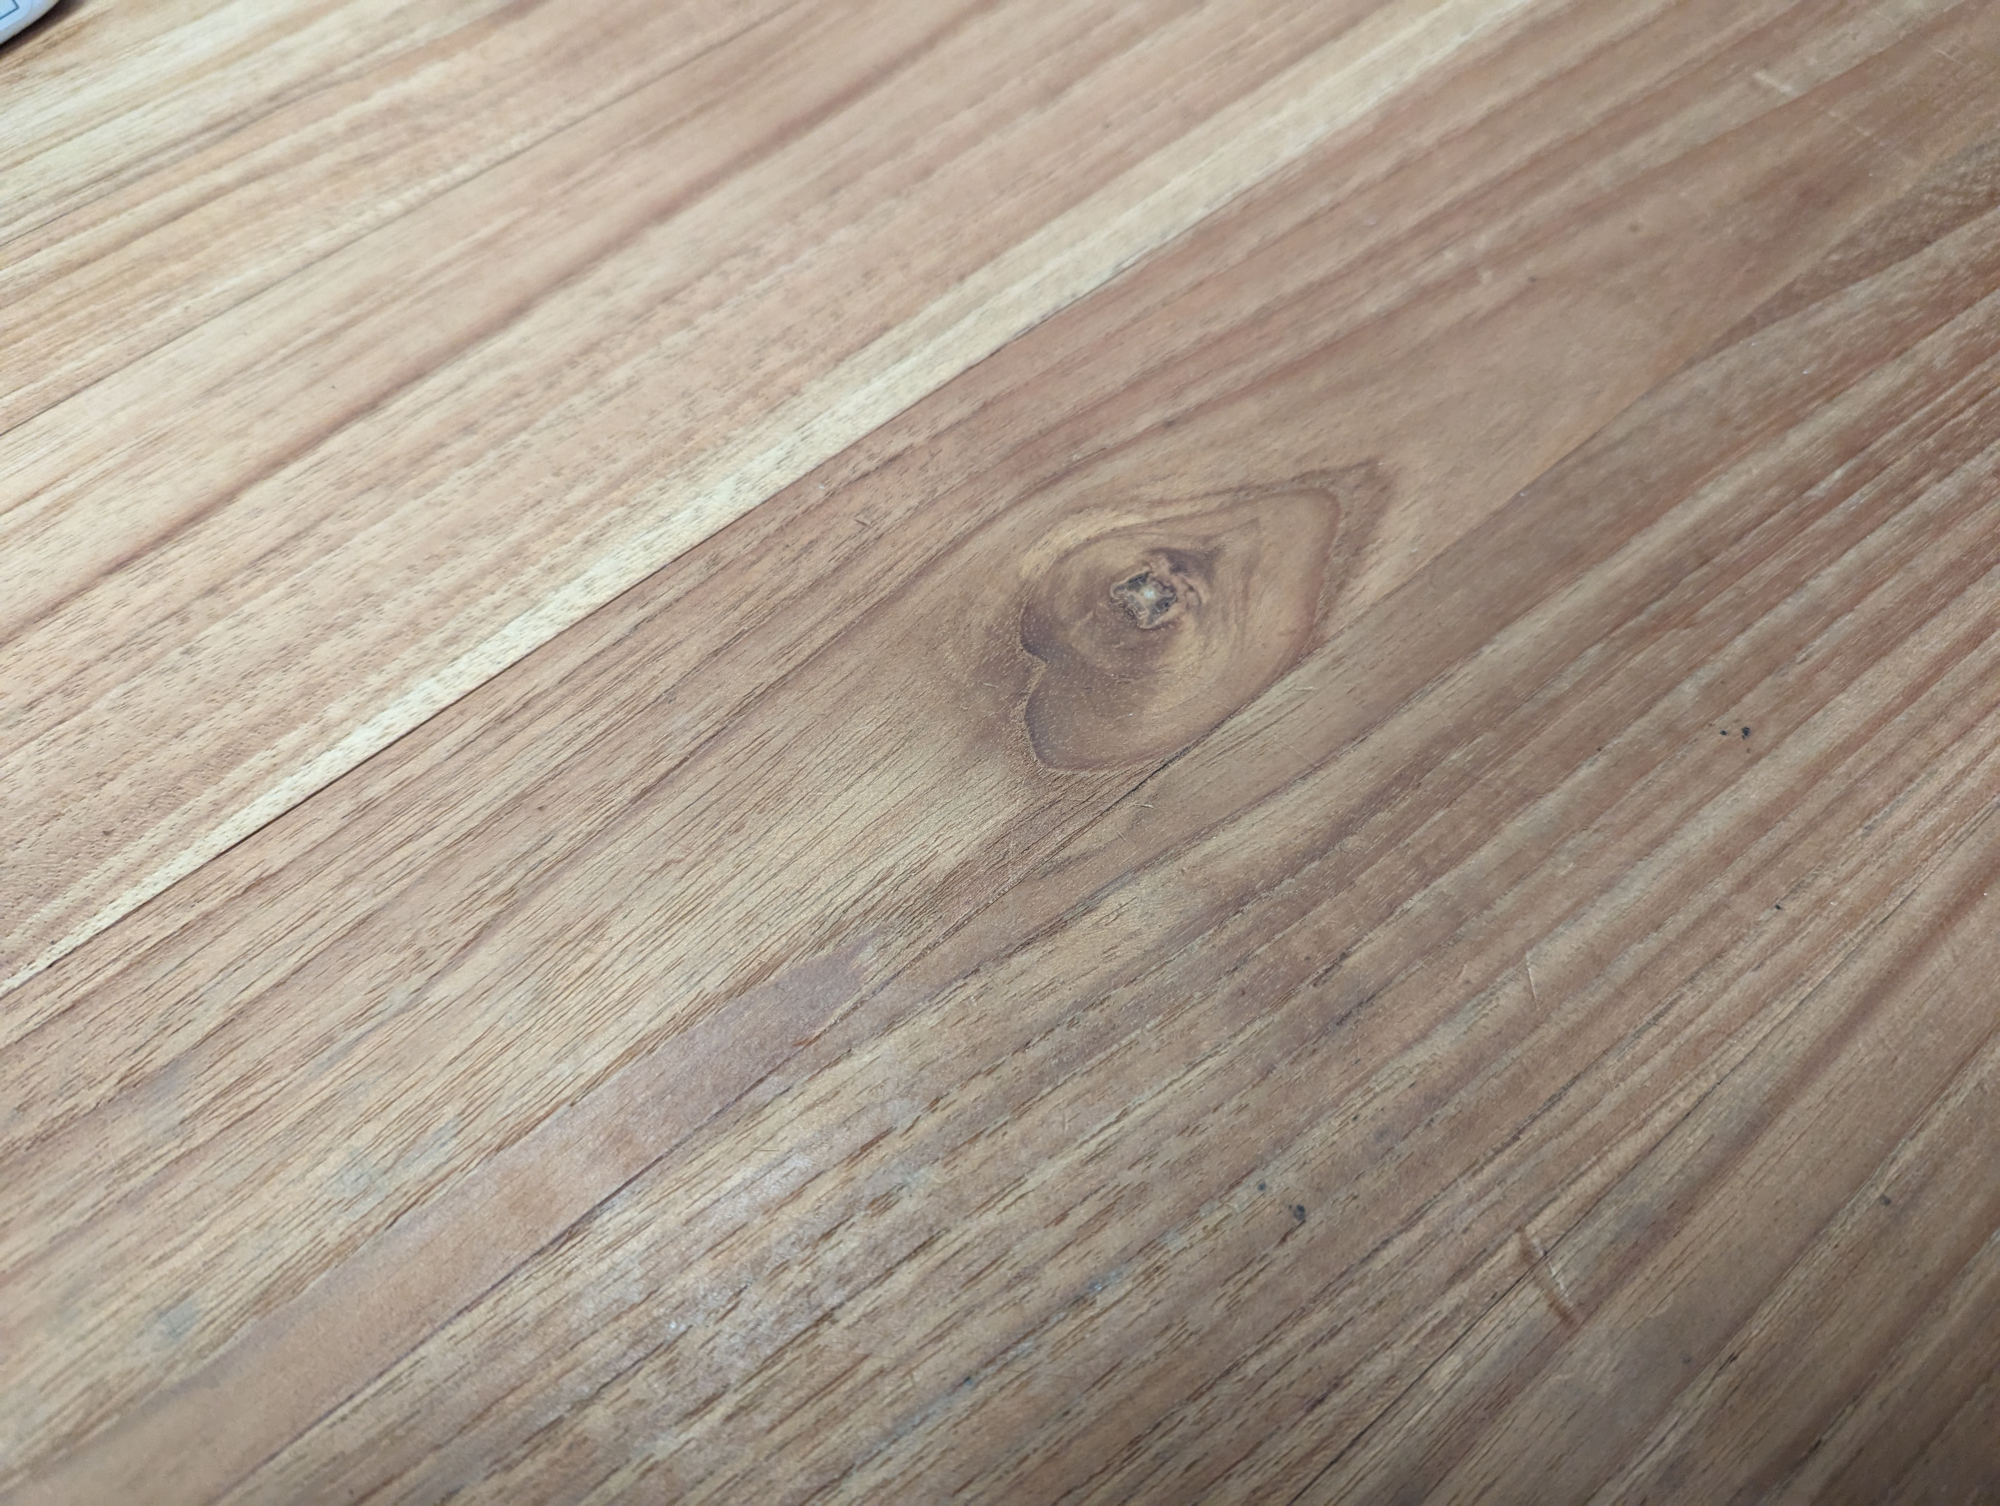
\includegraphics[width=0.8\linewidth]{../data/patchrefs/ref1}}
\caption{}
\label{fig:apples-d}
\end{subfigure}
\hfill
\begin{subfigure}{0.15\linewidth}
\fbox{\includegraphics[width=0.8\linewidth]{../data/patchimg}}
\caption{Hole version of \ref{fig:apples-a}}
\label{fig:apples-hole}
\end{subfigure}
\caption{The apple dataset}
\label{fig:apples}
\end{figure*}

\begin{figure*}
\centering
\hfill
\begin{subfigure}{0.15\linewidth}
\fbox{\includegraphics[width=0.8\linewidth]{../data/spongeinput}}
\caption{}
\label{fig:sponge-a}
\end{subfigure}
\hfill
\begin{subfigure}{0.15\linewidth}
\fbox{\includegraphics[width=0.8\linewidth]{../data/spongerefs/mpv-shot0001}}
\caption{}
\label{fig:sponge-b}
\end{subfigure}
\hfill
\begin{subfigure}{0.15\linewidth}
\fbox{\includegraphics[width=0.8\linewidth]{../data/spongerefs/mpv-shot0003}}
\caption{}
\label{fig:sponge-c}
\end{subfigure}
\hfill
\begin{subfigure}{0.15\linewidth}
\fbox{\includegraphics[width=0.8\linewidth]{../data/spongerefs/mpv-shot0004}}
\caption{}
\label{fig:sponge-d}
\end{subfigure}
\hfill
\begin{subfigure}{0.15\linewidth}
\fbox{\includegraphics[width=0.8\linewidth]{../data/spongerefs/mpv-shot0005}}
\caption{}
\label{fig:sponge-e}
\end{subfigure}
\hfill
\begin{subfigure}{0.15\linewidth}
\fbox{\includegraphics[width=0.8\linewidth]{../data/spongehole}}
\caption{Hole version of \ref{fig:sponge-a}}
\label{fig:sponge-hole}
\end{subfigure}
\caption{The Spongebob dataset}
\label{fig:sponge}
\end{figure*}

\begin{figure*}
\centering
\hfill
\begin{subfigure}{0.4\linewidth}
\fbox{\includegraphics[width=0.8\linewidth]{../data/basicOut1}}
\caption{Basic PatchMatch with \ref{fig:apples-a} as target and \ref{fig:apples-b} as source (PSNR: 77.50)}
\label{fig:applesbasic}
\end{subfigure}
\hfill
\begin{subfigure}{0.4\linewidth}
\fbox{\includegraphics[width=0.8\linewidth]{../data/refsOut3}}
\caption{Multiple reference PatchMatch with \ref{fig:apples-a} as target and the rest (excluding \ref{fig:apples-hole}) as source (PSNR: 78.33)}
\label{fig:applesrefs}
\end{subfigure}
\caption{Comparison of outputs of the PatchMatch algorithms on the apple dataset.}
\label{fig:applescompare}
\end{figure*}

\begin{figure*}
\centering
\hfill
\begin{subfigure}{0.4\linewidth}
\fbox{\includegraphics[width=0.8\linewidth]{../data/basicOut}}
\caption{Basic PatchMatch with \ref{fig:sponge-a} as target and \ref{fig:sponge-b} as source (PSNR: 81.16)}
\label{fig:spongebasic}
\end{subfigure}
\hfill
\begin{subfigure}{0.4\linewidth}
\fbox{\includegraphics[width=0.8\linewidth]{../data/refsOut}}
\caption{Multiple reference PatchMatch with \ref{fig:sponge-a} as target and the rest (excluding \ref{fig:sponge-hole}) as source (PSNR: 82.00)}
\label{fig:spongerefs}
\end{subfigure}
\caption{Comparison of outputs of the PatchMatch algorithms on the Spongebob dataset.}
\label{fig:spongecompare}
\end{figure*}

\begin{figure*}
\centering
\hfill
\begin{subfigure}{0.2\linewidth}
\fbox{\includegraphics[width=0.8\linewidth]{../data/scale0}}
\caption{Scale 0}
\label{fig:applescale0}
\end{subfigure}
\hfill
\begin{subfigure}{0.2\linewidth}
\fbox{\includegraphics[width=0.8\linewidth]{../data/scale1}}
\caption{Scale 1}
\label{fig:applescale1}
\end{subfigure}
\hfill
\begin{subfigure}{0.2\linewidth}
\fbox{\includegraphics[width=0.8\linewidth]{../data/scale2}}
\caption{Scale 2}
\label{fig:applescale2}
\end{subfigure}
\hfill
\begin{subfigure}{0.2\linewidth}
\fbox{\includegraphics[width=0.8\linewidth]{../data/fullOutput}}
\caption{Full output}
\label{fig:applefull}
\end{subfigure}
\caption{Progression of the hole fill on the apple dataset with \ref{fig:apples-hole} as target and the rest (excluding \ref{fig:apples-a}) as sources.}
\label{fig:applefill}
\end{figure*}

\begin{figure*}
\centering
\hfill
\begin{subfigure}{0.2\linewidth}
\fbox{\includegraphics[width=0.8\linewidth]{../data/scale0sponge}}
\caption{Scale 0}
\label{fig:spongescale0}
\end{subfigure}
\hfill
\begin{subfigure}{0.2\linewidth}
\fbox{\includegraphics[width=0.8\linewidth]{../data/scale1sponge}}
\caption{Scale 1}
\label{fig:spongescale1}
\end{subfigure}
\hfill
\begin{subfigure}{0.2\linewidth}
\fbox{\includegraphics[width=0.8\linewidth]{../data/scale2sponge}}
\caption{Scale 2}
\label{fig:spongescale2}
\end{subfigure}
\hfill
\begin{subfigure}{0.2\linewidth}
\fbox{\includegraphics[width=0.8\linewidth]{../data/fullOutputsponge}}
\caption{Full output}
\label{fig:spongefull}
\end{subfigure}
\caption{Progression of the hole fill on the Spongebob dataset with \ref{fig:sponge-hole} as target and the rest (excluding \ref{fig:sponge-a}) as sources.}
\label{fig:spongefill}
\end{figure*}

\begin{figure*}
\centering
\hfill
\begin{subfigure}{0.33\linewidth}
\fbox{\includegraphics[width=0.8\linewidth]{../data/efOut}}
\caption{My Efros Leung hole fill ($66\times50$ pixels)}
\label{fig:efapple}
\end{subfigure}
\hfill
\begin{subfigure}{0.33\linewidth}
\fbox{\includegraphics[width=0.8\linewidth]{../data/fullOutput}}
\caption{My PatchMatch hole fill ($266\times200$ pixels)}
\label{fig:pmapple}
\end{subfigure}
\begin{subfigure}{0.33\linewidth}
\fbox{\includegraphics[width=0.8\linewidth]{../data/img_cleanup}}
\caption{LaMa hole fill ($720\times542$ pixels)}
\label{fig:lamaapple}
\end{subfigure}
\caption{Comparison of hole fills on the apple dataset.}
\label{fig:applefillcompare}
\end{figure*}

\begin{figure*}
\centering
\hfill
\begin{subfigure}{0.45\linewidth}
\fbox{\includegraphics[width=0.8\linewidth]{../data/fullOutputsponge}}
\caption{My PatchMatch hole fill ($356\times200$ pixels)}
\label{fig:pmsponge}
\end{subfigure}
\hfill
\begin{subfigure}{0.45\linewidth}
\fbox{\includegraphics[width=0.8\linewidth]{../data/spongeinput_cleanup}}
\caption{LaMa hole fill ($720\times405$ pixels)}
\label{fig:lamasponge}
\end{subfigure}
\caption{Comparison of hole fills the Spongebob dataset.}
\label{fig:spongefillcompare}
\end{figure*}

\section{Background \& Related Work}
\label{sec:survey}

There are many existing algorithms that perform hole filling, also known as image inpainting. However, among the algorithms, none are applicable without modification to a situation containing multiple reference images. For this project, I chose to modify handcrafted algorithms rather than create a neural network. In this case, it's likely that handcrafted algorithms will be better able to use the few input images to create a better hole fill.

Of the existing handcrafted algorithms, I chose to modify the Efros-Leung and PatchMatch algorithm. The Efros-Leung algorithm is one of the first algorithms created capable of hole filling, while PatchMatch is one of the most recent hole filling algorithms. 

%-------------------------------------------------------------------------
\subsection*{Texture synthesis by non-parametric sampling \cite{efros1999texture}}

This paper by Efros and Leung describes a non-parametric sampling method for texture synthesis. The algorithm for texture synthesis starts by first copying a $3\times3$ pixel area from the source image into the center of an empty output image. Then, the blob is grown by scanning through the source image and copying pixels from the source image based on minimal distance, starting with the empty pixels with the most adjacent nonempty pixels. To perform hole filling, rather than beginning with a random patch of pixels, we begin with the input image containing a hole.

This method has a few disadvantages. First, it has a very poor runtime. The complexity of this algorithm is $O(n^2)$, since each of the $n$ pixels must compare windows with $n$ other pixels. Second, it is bad at preserving structures, since it operates on a greedy pixel by pixel basis. For example, this means that if we have a hole that intersects a flagpole, the flag pole may not be kept straight and connected in the output.s
\subsection*{PatchMatch: A randomized correspondence algorithm for structural image editing \cite{barnes2009patchmatch}}
This paper by Barnes \etal describes the PatchMatch algorithm which generates images by copying patches from the input. In the basic PatchMatch algorithm, we have a target image to be generated from patches in a separate source image.

The first step of the algorithm is to randomly initialize a nearest neighbor field (NNF), which contains vectors from the target image to the source image. The NNF is then iteratively improved through propagation and random search. Five iterations are enough to converge to an ideal output.

During propagation, each pixel compares its own vector to the vectors of its neighbors in scanline or reverse scanline order. If a neighbor's vector results in a lower distance between the target window and the source window, then the pixel sets its own vector to the vector of its neighbor. In this way, a single correct random vector can be passed along to all other nearby pixels in a similar patch.

The random search steps helps the algorithm escape from local minima. After each instance of propagation, the pixel will consider a random vector to a point in the source image within an exponentially shrinking radius. By the same probabilistic principle that allows for a random initialization, this random search also has a high likelihood of escaping from local minima.

Compared to Efros-Leung, the complexity of this algorithm is much lower at only $O(n\log n)$. Since it operates on patches of pixels rather than single pixels, it is also likely to preserve structures.
\subsection*{Synthesizing natural textures \cite{ashikhmin2001synthesizing}}
This paper by Ashikhmin describes an algorithm which outspeeds the Efros Leung algorithm by encouraging copying of larger patches from the input image. This algorithm is similar to the quilting algorithm described in Homework 2, however the patches are irregularly shaped, which makes it better suited for natural textures. This is one of the papers cited by the PatchMatch paper, but I ultimately chose not to use it.
\subsection*{Region filling and object removal by exemplar-based image inpainting \cite{criminisi2004region}}
This paper by Criminisi \etal describes an algorithm which works for filling both small and large holes in images. The algorithm works by filling patches of the hole in order of highest priority, determined by the level of confidence in filling the patch, to avoid artifacting. I ended up not using this paper.
\subsection*{Resolution-robust Large Mask Inpainting with Fourier Convolutions \cite{suvorov2022resolution}}
This paper describes a modern neural network based image inpainting algorithm called large mask inpainting (LaMa) which uses fast Fourier convolutions to improve the efficacy of hole filling. I will use this as a comparison for my handcrafted algorithms.